\documentclass[a4paper]{article}
\usepackage{amsmath}
\usepackage{amssymb}
\usepackage{amsthm}
\usepackage{siunitx}
\usepackage{enumitem}
\usepackage{undertilde}
\usepackage{tikz} % Package for drawing
\usepackage{pgfplots}
\usepgfplotslibrary{fillbetween} %%% fill between
\usepackage[margin=1.5cm]{geometry}
\renewcommand{\familydefault}{\sfdefault} %% sans font as a default 
\newcommand{\ee}{\mathrm{e}}
\newcommand{\dd}{\mathrm{d}}
\newcommand{\id}{\mathrm{\,d}}
\newcommand{\ii}{\mathrm{i}}
\newcommand{\rp}{\mathrm{Re\,}}
\newcommand{\ip}{\mathrm{Im\,}}
\newcommand{\vi}{\mathbf{i}}
\newcommand{\vj}{\mathbf{j}}
\newcommand{\vk}{\mathbf{k}}
\newcommand{\DAG}{(\textbf{\dag})\ }
\setlength{\parindent}{0mm}
%\newtheorem{qz}{Quiz}
%\newcommand{\quiz}{\begin{qz}\end{qz}}   Alan's assignment ---- assignment
\pagestyle{empty}
\newtheorem{asm}{\textbf{\large Assignment}}
\newcommand{\assignment}{\begin{asm}\end{asm}}

%\pgfplotsset{every axis/.append style={
%%		axis x line=middle,    % put the x axis in the middle
%		axis y line=middle,    % put the y axis in the middle
%		axis line style={->}, % arrows on the axis
%		axis equal,
%		xmajorticks=false, 	 
%		ymajorticks=false,
%		%	unit vector ratio*=1 1 1,
%%		enlarge y limits=true,
%		xlabel={$x$},
%		ylabel={$y$},
%		x label style={=at={((current axis.right of origin)), anchor=north},right =0.8mm},	
%		y label style={=at={(current axis.up of origin), anchor=north}}	
%}}


\begin{document} 
                               %%%%%%%%%%%%%%%%%%%%%%%%%%%%%%%%%%%%%%%%%%%%
\assignment                    %%%   Assignment 1 Representation of data %%%
                               %%%%%%%%%%%%%%%%%%%%%%%%%%%%%%%%%%%%%%%%%%%%
\begin{enumerate}
    %%%%%%%%%%%%%%%%%%%%%%%%%%%%%%%%%%%%%
	%%%%%%%%%%%%%%%%%%%%%%%%%%%%%%%%%%%%%
	%%%%%%%%%%%%%%%%%%%%%%%%%%%%%%%%%%%%%
	%%% Question 1  9709 s17 qp62  Q2 %%%%
	%%%%%%%%%%%%%%%%%%%%%%%%%%%%%%%%%%%%%
	%%%%%%%%%%%%%%%%%%%%%%%%%%%%%%%%%%%%%
	%%%%%%%%%%%%%%%%%%%%%%%%%%%%%%%%%%%%%
	\item Anabel measured the lengths, in centimetres, of $200$ caterpillars. Her results are illustrated in the	cumulative frequency graph below.
	
	\medskip
	
	
	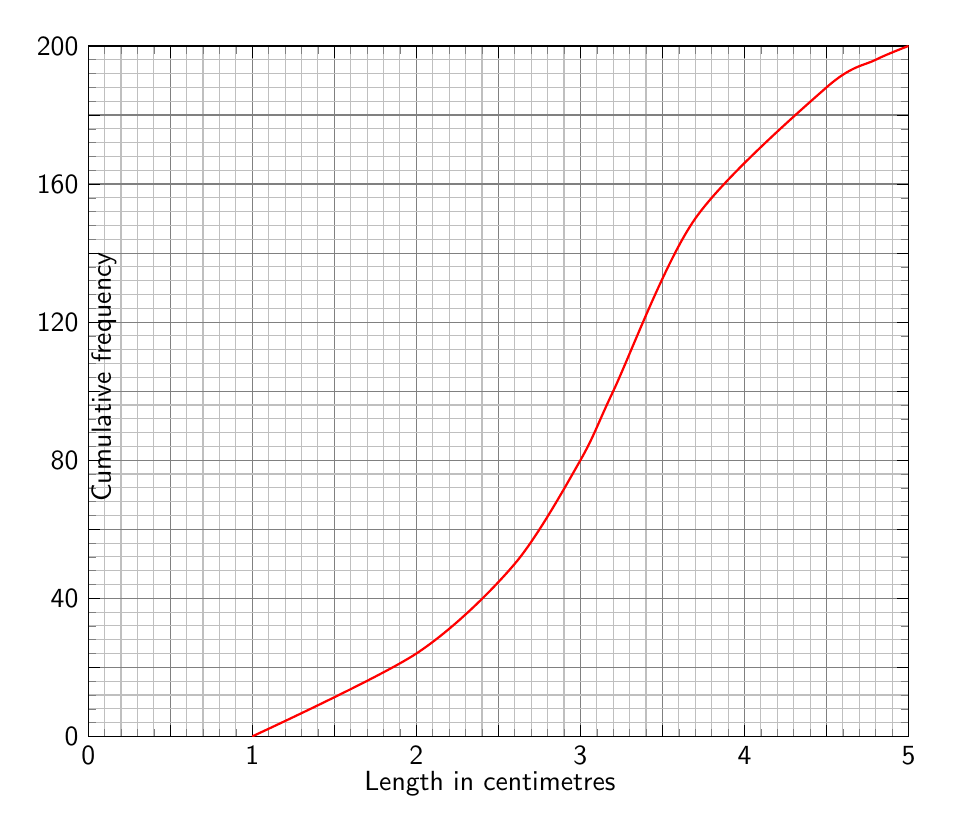
\begin{tikzpicture}
		\centering
		
		\begin{axis}[
			width = 12cm,
			%axis x line = middle,
			xmin = 0, xmax=5,
			ymin=0, ymax= 200,
			grid = both,
			minor grid style=lightgray,
			ytick={0,20,40,60,80,
				100,120,140,160,180,
				200},
			yticklabels={0,\empty,40,\empty,80,
				\empty,120,\empty,160,\empty,
				200
			},
			xtick={0,0.5,1,1.5,2,
				2.5,3,3.5,4,4.5,
				5},
			xticklabels={0,\empty,1,\empty,2,
				\empty,3,\empty,4,\empty,
				5},
			major grid style =gray,
			major tick style=black,	
			minor x tick num=4,
			minor y tick num=4, 
			%extra x ticks={5,15,25,35,45,},
			%extra x tick labels={5,15,25,35,45},
			%extra y ticks={5,15,25,35,45,55},
			%extra y tick labels={\empty,\empty,\empty,\empty,\empty},
			%extra tick style={
			%	tick style=thick
			%},	
			%yticklabels={\empty,\empty,\empty},
			x label style={at={(current axis.right of origin)},anchor=north, below=0.6cm, left =3.6cm},
			y label style={at={(current axis.above origin)},anchor = west, below =2mm,left = 25mm},
			xlabel={Length in centimetres},
			ylabel={Cumulative frequency}
			]	
			\addplot[thick, mark=none,smooth,red] plot coordinates { 
				(1,0)
				(2,24)
				(2.6,50)		
				(3,80)
				(3.2,100)
				(3.7,150)
				(4.5,188)
				(4.8,196)
				(5,200)
				
			} ;	
			
		\end{axis}
	\end{tikzpicture}
	
	\medskip
	
	\begin{enumerate}[label=(\roman*)]
		\item Estimate the median and the interquartile range of the lengths. \hfill [3]
		
		\vspace{3cm}
		
		\item Estimate how many caterpillars had a length of between $2$ and $3.5$ \si{\cm}. \hfill [1]
		
		\vspace{3cm}
		\item $6\%$ of caterpillars were of length $l$ centimetres or more. Estimate $l$. \hfill [2]
		
		\vspace{4cm}
		
		
	\end{enumerate}
	\clearpage
	%%%%%%%%%%%%%%%%%%%%%%%%%%%%%%%%%%%%%
	%%%%%%%%%%%%%%%%%%%%%%%%%%%%%%%%%%%%%
	%%%%%%%%%%%%%%%%%%%%%%%%%%%%%%%%%%%%%
	%%% Question 2  9709 w18 qp63  Q7 %%%%
	%%%%%%%%%%%%%%%%%%%%%%%%%%%%%%%%%%%%%
	%%%%%%%%%%%%%%%%%%%%%%%%%%%%%%%%%%%%%
	%%%%%%%%%%%%%%%%%%%%%%%%%%%%%%%%%%%%%
	
	\item 
	
	
	
	The heights, in \si{\cm}, of the $11$ members of the Anvils athletics team and the $11$ members of the Brecons swimming team are shown below.
	
	\medskip
	
	\renewcommand{\arraystretch}{1.2} % default is 1.0
	\begin{tabular}{|l|c|c|c|c|c|c|c|c|c|c|c|}
		\hline
		Anvils  & $ 173 $ & $ 158 $ & $ 180 $ & $ 196$ & $175 $  & $165$ & $170$ & $169$& $181$& $184$ & $172$ \\ 
		\hline
		Brecons & $ 166 $ & $ 170 $ & $ 171 $ & $ 172$ & $172 $  & $178$ & $181$ & $182$& $183$& $183$ & $192$ \\ 
		\hline
	\end{tabular}
	
	\medskip
	
	\begin{enumerate}[label=(\roman*)]
		\item Draw a back-to-back stem-and-leaf diagram to represent this information, with Anvils on the
		left-hand side of the diagram and Brecons on the right-hand side. \hfill [4]
		
		\vspace{8cm}
		
		\item Find the median and the interquartile range for the heights of the Anvils. \hfill [3]
		
		\vspace{6cm}
	\end{enumerate}
	
	The heights of the $11$ members of the Anvils are denoted by $x$ \si{\cm}. It is given that $ \sum x =1923$, and  $\sum x^2 =337 221$. Suppose the Anvils are joined by $3$ new members whose heights are $166$ \si{\cm}, $172$ \si{\cm} and $182$ \si{\cm}.
	
	\begin{enumerate}[resume,label=(\roman*)]
		\item Find the standard deviation of the heights of all $14$ members of the Anvils.\hfill  [4]
		
		\vspace{5cm}
	\end{enumerate}
	
	\clearpage
	%%%%%%%%%%%%%%%%%%%%%%%%%%%%%%%%%%%%%
	%%%%%%%%%%%%%%%%%%%%%%%%%%%%%%%%%%%%%
	%%%%%%%%%%%%%%%%%%%%%%%%%%%%%%%%%%%%%
	%%% Question 3  9709 w19 qp62  Q3 %%%%
	%%%%%%%%%%%%%%%%%%%%%%%%%%%%%%%%%%%%%
	%%%%%%%%%%%%%%%%%%%%%%%%%%%%%%%%%%%%%
	%%%%%%%%%%%%%%%%%%%%%%%%%%%%%%%%%%%%%
	
	\item  The speeds, in \si{\km\per\hour}, of $90$ cars as they passed a certain marker on a road were recorded, correct to the nearest \si{\km\per\hour}. The results are summarised in the following table.
	
	
	\medskip
	
	\renewcommand{\arraystretch}{1.2} % default is 1.0
	\begin{tabular}{|l|c|c|c|c|c|}
		\hline
		Speeds (\si{\km\per\hour})  & $ 10-29 $ & $ 30-39 $ & $ 40-49 $ & $ 50-59$ & $60-89$ \\ 
		\hline
		Frequency & $ 10$ & $ 24 $ & $ 30$ & $ 14$ & $12 $ \\ 
		\hline
	\end{tabular}
	
	\medskip
	
	\begin{enumerate}[label=(\roman*)]
		\item On the grid, draw a histogram to illustrate the data in the table. \hfill [4]
		
		\vspace{5cm}
		
		\medskip	
		
		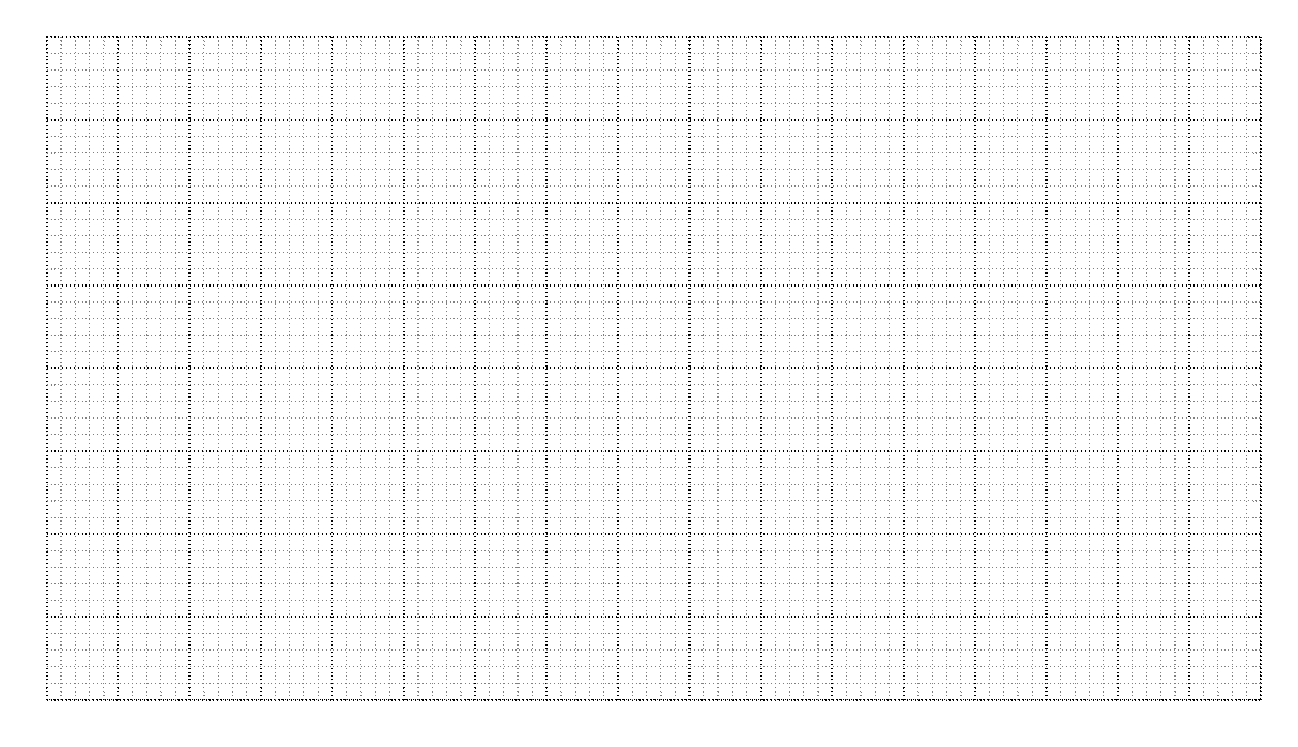
\begin{tikzpicture}
			\centering
			
			\begin{axis}[densely dotted,
				grid = both,
				minor grid style=gray,
				major grid style =black,
				major grid style ={line width =0.8pt},
				%	major grid style =thick,
				major tick style=black,	
				width = 17cm,	
				height = 10cm,		
				%axis x line = middle,
				xmin = 0, xmax=17,
				ymin=0, ymax= 8,			
				ytick={0,1,2,3,4,5,6,7,8},
				yticklabels={\empty,\empty,\empty,\empty,\empty,
					\empty,\empty,\empty,\empty
				},
				xtick={0,1,2,3,4,5,6,7,8,9,10,11,12,13,14,15,16,17},
				xticklabels={\empty,\empty,\empty,\empty,
					\empty,\empty,\empty,\empty,
					\empty,\empty,\empty,\empty,
					\empty,\empty,\empty,\empty,
					\empty,\empty
				},			
				minor x tick num=4,
				minor y tick num=4, 
				%extra x ticks={5,15,25,35,45,},
				%extra x tick labels={5,15,25,35,45},
				%extra y ticks={5,15,25,35,45,55},
				%extra y tick labels={\empty,\empty,\empty,\empty,\empty},
				%extra tick style={
				%	tick style=thick
				%},	
				%yticklabels={\empty,\empty,\empty},
				x label style={at={(current axis.right of origin)},anchor=north, below=0.4cm, left =3.6cm},
				y label style={at={(current axis.above origin)},anchor = west, below =0.5mm,left = 30mm},
				xlabel={},
				ylabel={}
				]	
				
			\end{axis}
		\end{tikzpicture}
		
		\vspace{2cm}
		\item Calculate an estimate for the mean speed of these $90$ cars as they pass the marker. \hfill [2]
		
		\vspace{5cm}
	\end{enumerate}
	
	\clearpage
	%%%%%%%%%%%%%%%%%%%%%%%%%%%%%%%%%%%%%
	%%%%%%%%%%%%%%%%%%%%%%%%%%%%%%%%%%%%%
	%%%%%%%%%%%%%%%%%%%%%%%%%%%%%%%%%%%%%
	%%% Question 4  9709 s18 qp63  Q4 %%%%
	%%%%%%%%%%%%%%%%%%%%%%%%%%%%%%%%%%%%%
	%%%%%%%%%%%%%%%%%%%%%%%%%%%%%%%%%%%%%
	%%%%%%%%%%%%%%%%%%%%%%%%%%%%%%%%%%%%%
	
	\item  Farfield Travel and Lacket Travel are two travel companies which arrange tours abroad. The numbers
	of holidays arranged in a certain week are recorded in the table below, together with the means and
	standard deviations of the prices.
	
	\medskip
	
	\begin{table}[!htpb]
		\centering
		\renewcommand{\arraystretch}{1.2} % default is 1.0
		\begin{tabular}{l|c|c|c|}
			\cline{2-4}
			& Number of holidays & Mean price ($\$$) & Standard deviation ($\$$) \\ \hline
			\multicolumn{1}{|l|}{Farfield Travel} & $30$                 & $1500$            & $230 $                    \\ \hline
			\multicolumn{1}{|l|}{Lacket Travel}   & $21$                 & $2400 $           & $160  $                   \\ \hline
		\end{tabular}
	\end{table}
	
	\medskip
	
	\begin{enumerate}[label=(\roman*)]
		\item Calculate the mean price of all $51$ holidays. \hfill [2]
		
		\vspace{4cm}
		\item The prices of individual holidays with Farfield Travel are denoted by $\$ x_F$	and the prices of
		individual holidays with Lacket Travel are denoted by $\$x_L$. By first finding $\sum x_F^2$ and  $\sum x_L^2$, find the standard deviation of the prices of all $51$ holidays. \hfill[5]
	\end{enumerate}
	
	\clearpage
	%%%%%%%%%%%%%%%%%%%%%%%%%%%%%%%%%%%%%
	%%%%%%%%%%%%%%%%%%%%%%%%%%%%%%%%%%%%%
	%%%%%%%%%%%%%%%%%%%%%%%%%%%%%%%%%%%%%
	%%% Question 5  9709 s19 qp61  Q4 %%%%
	%%%%%%%%%%%%%%%%%%%%%%%%%%%%%%%%%%%%%
	%%%%%%%%%%%%%%%%%%%%%%%%%%%%%%%%%%%%%
	%%%%%%%%%%%%%%%%%%%%%%%%%%%%%%%%%%%%%
	
	\item The Mathematics and English A-level marks of $1400$ pupils all taking the same examinations are
	shown in the cumulative frequency graphs below. Both examinations are marked out of $100$.
	
	\medskip
	
	
	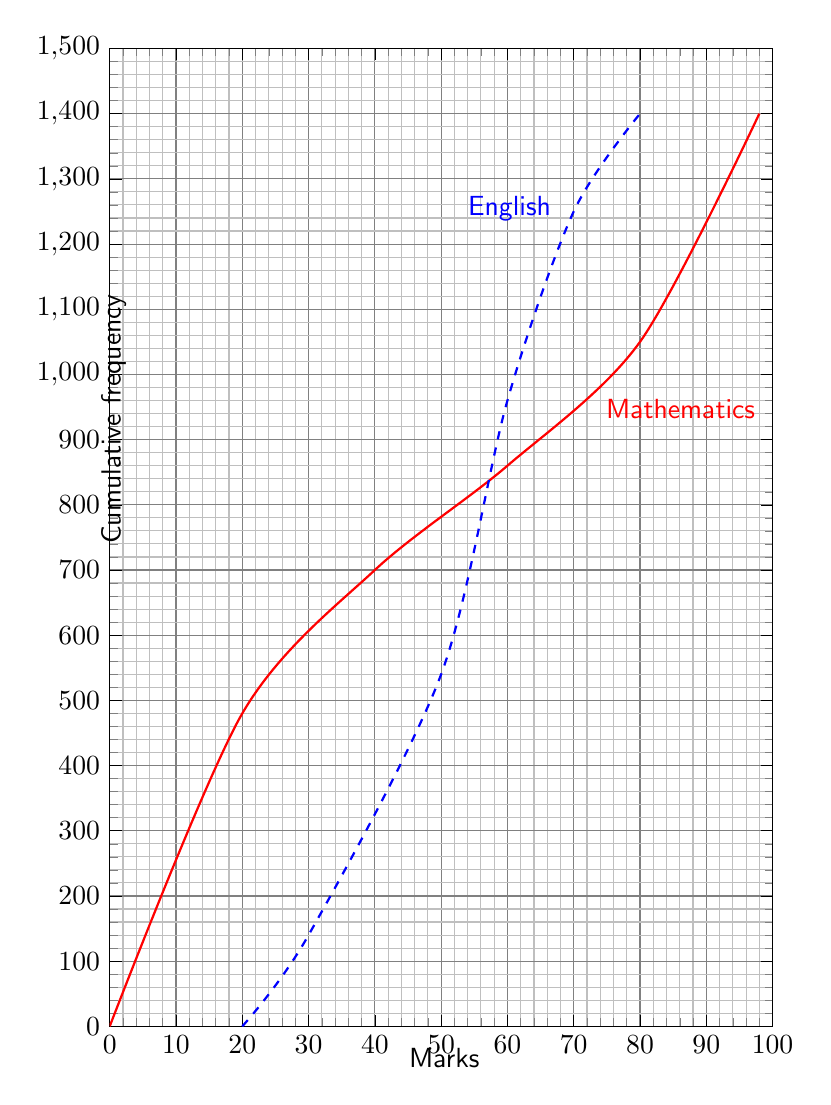
\begin{tikzpicture}
		\centering
		
		\begin{axis}[
			width = 10cm,
			height = 14cm,
			%axis x line = middle,
			xmin = 0, xmax=100,
			ymin=0, ymax= 1500,
			grid = both,
			minor grid style=lightgray,
			ytick={0,100,200,300,400,
				500,600,700,800,900,
				1000,1100,1200,1300,1400,1500},
			%	yticklabels={0,\empty,40,\empty,80,
			%		\empty,120,\empty,160,\empty,
			%		200
			%	},
			xtick={0,10,20,30,40,50,
				60,70,80,90,100},
			%	xticklabels={0,\empty,1,\empty,2,
			%		\empty,3,\empty,4,\empty,
			%		5},
			major grid style =gray,
			major tick style=black,	
			minor x tick num=4,
			minor y tick num=4, 
			%extra x ticks={5,15,25,35,45,},
			%extra x tick labels={5,15,25,35,45},
			%extra y ticks={5,15,25,35,45,55},
			%extra y tick labels={\empty,\empty,\empty,\empty,\empty},
			%extra tick style={
			%	tick style=thick
			%},	
			%yticklabels={\empty,\empty,\empty},
			x label style={at={(current axis.right of origin)},anchor=north, below=0.4cm, left =3.6cm},
			y label style={at={(current axis.above origin)},anchor = west, below =0.5mm,left = 30mm},
			xlabel={Marks},
			ylabel={Cumulative frequency}
			]	
			\addplot[thick, mark=none,smooth,red] plot coordinates { 
				(0,0)
				%	(2,100)
				(20,480)
				%	(30,600)
				(40,700)
				(60,860)
				(80,1050)
				(98,1400)			
			} node[below,yshift=-3.5cm,xshift=-1cm]{Mathematics};	
			\addplot[thick, mark=none,smooth,blue,dashed] plot coordinates { 
				(20,0)
				%	(2,100)
				(30,140)
				%	(30,600)
				(50,540)
				(60,960)
				(70,1250)
				(80,1400)			
			}node[left,xshift=-1.0cm,yshift=-1.2cm]{English} ;	
			
		\end{axis}
	\end{tikzpicture}
	
	Use suitable data from these graphs to compare the central tendency and spread of the marks in
	Mathematics and English. \hfill [6]
	
	\clearpage
	%%%%%%%%%%%%%%%%%%%%%%%%%%%%%%%%%%%%%
	%%%%%%%%%%%%%%%%%%%%%%%%%%%%%%%%%%%%%
	%%%%%%%%%%%%%%%%%%%%%%%%%%%%%%%%%%%%%
	%%% Question 6  9709 w18 qp62  Q2 %%%%
	%%%%%%%%%%%%%%%%%%%%%%%%%%%%%%%%%%%%%
	%%%%%%%%%%%%%%%%%%%%%%%%%%%%%%%%%%%%%
	%%%%%%%%%%%%%%%%%%%%%%%%%%%%%%%%%%%%%
	
	\item The following back-to-back stem-and-leaf diagram shows the reaction times in seconds in an
	experiment involving two groups of people, $A$ and $B$.
	
	\begin{table}[!htpb]
		\centering
		\setlength{\tabcolsep}{2.2mm}  %% set column width of a table
		\begin{tabular}{cllllllll|l|cllllllll}
			\multicolumn{9}{c|}{$A$}              &    & \multicolumn{9}{c}{$B$}               \\ \hline
			(4) &   &   &   &   & 4 & 2 & 0 & 0 & 20 & 5 & 6 & 7 &   &   &   &   &   & (3) \\
			(5) &   &   &   & 9 & 8 & 5 & 0 & 0 & 21 & 1 & 2 & 2 & 3 & 7 & 7 &   &   & (6) \\
			(8) & 9 & 8 & 7 & 5 & 3 & 2 & 2 & 2 & 22 & 1 & 3 & 5 & 6 & 6 & 8 & 9 &   & (7) \\
			(6) &   &   & 8 & 7 & 6 & 5 & 2 & 1 & 23 & 4 & 5 & 7 & 8 & 8 & 9 & 9 & 9 & (8) \\
			(3) &   &   &   &   &   & 8 & 6 & 3 & 24 & 2 & 4 & 5 & 6 & 7 & 8 & 8 &   & (7) \\
			(1) &   &   &   &   &   &   &   & 0 & 25 & 0 & 2 & 7 & 8 &   &   &   &   & (4)
		\end{tabular}
		
		\vspace{4 pt}
		
		
		\fbox{\parbox{4.8in}{Key:  $5 |22|6$ means a reaction time of $0.225$ seconds for $A$ and $0.226$ seconds for $B$}}
	\end{table}
	
	\begin{enumerate}[label=(\roman*)]
		\item Find the median and the interquartile range for group $A$. \hfill[3]
		
		\vspace{4cm}
		
	\end{enumerate}
	
	The median value for group $B$ is $0.235$ seconds, the lower quartile is $0.217$ seconds and the upper
	quartile is $0.245$ seconds.
	
	\begin{enumerate}[resume,label=(\roman*)]
		\item Draw box-and-whisker plots for groups $A$ and $B$ on the grid. \hfill [3]
		
		
		\medskip
		\vspace{1cm}
		
		
		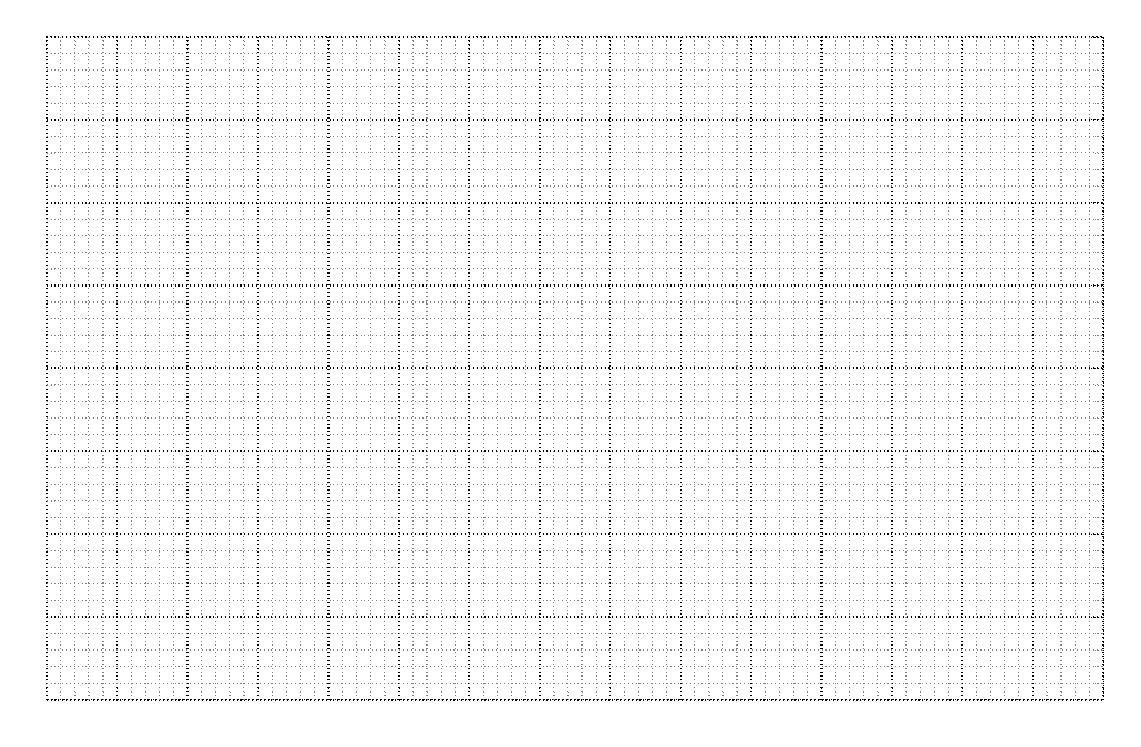
\begin{tikzpicture}
			\centering
			
			\begin{axis}[densely dotted,
				grid = both,
				minor grid style=gray,
				major grid style =black,
				major grid style ={line width =0.8pt},
				%	major grid style =thick,
				major tick style=black,	
				width = 15cm,	
				height = 10cm,		
				%axis x line = middle,
				xmin = 0, xmax=15,
				ymin=0, ymax= 8,			
				ytick={0,1,2,3,4,5,6,7,8},
				yticklabels={\empty,\empty,\empty,\empty,\empty,
					\empty,\empty,\empty,\empty
				},
				xtick={0,1,2,3,4,5,6,7,8,9,10,11,12,13,14,15},
				xticklabels={\empty,\empty,\empty,\empty,
					\empty,\empty,\empty,\empty,
					\empty,\empty,\empty,\empty,
					\empty,\empty,\empty,\empty
				},			
				minor x tick num=4,
				minor y tick num=4, 
				%extra x ticks={5,15,25,35,45,},
				%extra x tick labels={5,15,25,35,45},
				%extra y ticks={5,15,25,35,45,55},
				%extra y tick labels={\empty,\empty,\empty,\empty,\empty},
				%extra tick style={
				%	tick style=thick
				%},	
				%yticklabels={\empty,\empty,\empty},
				x label style={at={(current axis.right of origin)},anchor=north, below=0.4cm, left =3.6cm},
				y label style={at={(current axis.above origin)},anchor = west, below =0.5mm,left = 30mm},
				xlabel={},
				ylabel={}
				]	
				
			\end{axis}
		\end{tikzpicture}
	\end{enumerate}
	
\end{enumerate} 
	\vspace{1cm}
	\vfill
\textbf{Total mark} of this assignment: $41$.\\

%The symbol \DAG indicates a bonus question. Finish other questions before working on this one.\\

\clearpage 

                               %%%%%%%%%%%%%%%%%%%%%%%%%%%%%%%%%%%%%%%%%%%%%%%%%%
\assignment                    %%%   Assignment 2 Permutation and Combination %%%
                               %%%%%%%%%%%%%%%%%%%%%%%%%%%%%%%%%%%%%%%%%%%%%%%%%%

\begin{enumerate}
	
	%%%%%%%%%%%%%%%%%%%%%%%%
	%%%%%%%%%%%%%%%%%%%%%%%%
	%%% Q1 s18_qp_61_7 %%%%%
	%%%%%%%%%%%%%%%%%%%%%%%%
	%%%%%%%%%%%%%%%%%%%%%%%%
	%%%%%%%%%%%%%%%%%%%%%%%%	
	
	\item Find the number of different ways in which all $9$ letters of the word \textbf{MINCEMEAT} can be arranged in	each of the following cases. 
	\begin{enumerate}[label=(\roman*)]
		\item There are no restrictions.  \hfill[1]
		\vspace{2cm}
		\item No vowel (\textbf{A}, \textbf{E}, \textbf{I} are vowels) is next to another vowel. \hfill[4]
		
		\vspace{2cm}
	\end{enumerate}
	$5$ of the $9$ letters of the word \textbf{MINCEMEAT} are selected.
	\begin{enumerate}[resume,label=(\roman*)]
		\item Find the number of possible selections which contain exactly $1$ \textbf{M} and exactly $1$ \textbf{E}. \hfill[2]
		\vspace{2cm}
		\item  Find the number of possible selections which contain at least $1$ \textbf{M} and at least $1$ \textbf{E}. \hfill[3]
		\vspace{2cm}
	\end{enumerate}
	
	
	
	%%%%%%%%%%%%%%%%%%%%%%%%
	%%%%%%%%%%%%%%%%%%%%%%%%
	%%% Q2 s18_qp_62_6 %%%%%
	%%%%%%%%%%%%%%%%%%%%%%%%
	%%%%%%%%%%%%%%%%%%%%%%%%
	%%%%%%%%%%%%%%%%%%%%%%%%
	
	\item  \begin{enumerate}[label=(\roman*)]
		\item Find the number of ways in which all $9$ letters of the word \textbf{AUSTRALIA} can be arranged in each of the following cases.
		
		\begin{enumerate}[label=(\alph*)]
			\item All the vowels (\textbf{A}, \textbf{I}, \textbf{U} are vowels) are together. \hfill [3]
			\vspace{3cm}
			\item The letter \textbf{T} is in the central position and each end position is occupied by one of the other consonants (\textbf{R}, \textbf{S}, \textbf{L}). \hfill [3]
			\vspace{3cm}
		\end{enumerate}
		\item Donna has $2$ necklaces, $8$ rings and $4$ bracelets, all different. She chooses $4$ pieces of jewellery.
		
		How many possible selections can she make if she chooses at least $1$ necklace and at least $1$ 	bracelet?  \hfill [4]
		\vspace{4cm}
	\end{enumerate}
	
	
	%%%%%%%%%%%%%%%%%%%%%%%%
	%%%%%%%%%%%%%%%%%%%%%%%%
	%%% Q3 s18_qp_63_7 %%%%%
	%%%%%%%%%%%%%%%%%%%%%%%%
	%%%%%%%%%%%%%%%%%%%%%%%%
	%%%%%%%%%%%%%%%%%%%%%%%%
	
	\item Find the number of ways the $9$ letters of the word \textbf{SEVENTEEN} can be arranged in each of the following cases.
	
	\begin{enumerate}[label=(\roman*)]
		\item One of the letter \textbf{E}s is in the centre with $4$ letters on either side. \hfill[2]
		\vspace{2cm}
		\item No \textbf{E} is next to another \textbf{E}. \hfill[3]
		\vspace{2cm}
	\end{enumerate}
	$5$ letters are chosen from the $9$ letters of the word \textbf{SEVENTEEN}.
	\begin{enumerate}[resume,label=(\roman*)]
		\item Find the number of possible selections which contain exactly $2$ \textbf{E}s and exactly 2 \textbf{N}s. \hfill[1]
		\vspace{2cm}
		\item Find the number of possible selections which contain at least $2$ \textbf{E}s. \hfill[4]
		\vspace{2cm}
	\end{enumerate}
	
	%%%%%%%%%%%%%%%%%%%%%%%%
	%%%%%%%%%%%%%%%%%%%%%%%%
	%%% Q4 s19_qp_61_7 %%%%%
	%%%%%%%%%%%%%%%%%%%%%%%%
	%%%%%%%%%%%%%%%%%%%%%%%%
	%%%%%%%%%%%%%%%%%%%%%%%%
	
	\item  Freddie has $6$ toy cars and $3$ toy buses, all different. He chooses $4$ toys to take on holiday with him.
	
	\begin{enumerate}[label=(\roman*)]
		\item In how many different ways can Freddie choose $4$ toys? \hfill[1]
		\vspace{2cm}
		\item How many of these choices will include both his favourite car and his favourite bus? \hfill[2]
		\vspace{2cm}
	\end{enumerate}
	
	Freddie arranges these $9$ toys in a line.
	
	\begin{enumerate}[resume,label=(\roman*)]
		\item Find the number of possible arrangements if the buses are all next to each other. \hfill[3]
		\vspace{3cm}
		\item  Find the number of possible arrangements if there is a car at each end of the line and no buses are next to each other. \hfill[3]
		\vspace{3cm}
	\end{enumerate}
	
	
	%%%%%%%%%%%%%%%%%%%%%%%%
	%%%%%%%%%%%%%%%%%%%%%%%%
	%%% Q5 s19_qp_62_7 %%%%%
	%%%%%%%%%%%%%%%%%%%%%%%%
	%%%%%%%%%%%%%%%%%%%%%%%%
	%%%%%%%%%%%%%%%%%%%%%%%%
	
	\item  \begin{enumerate}[label=(\roman*)]
		\item A group of $6$ teenagers go boating. There are three boats available. One boat has room for $3$ people, one has room for $2$ people and one has room for $1$ person. Find the number of different ways the group of 6 teenagers can be divided between the three boats.\hfill [3]
		\vspace{2cm}
		\item Find the number of different $7$-digit numbers which can be formed from the seven digits $2$, $2$, $3$, $7$, $7$, $7$, $8$ in each of the following cases.
		\begin{enumerate}[label=(\alph*)]
			\item The odd digits are together and the even digits are together. \hfill [3]
			\vspace{2cm}
			\item The $2$s are not together. \hfill[4]
			\vspace{2cm}
		\end{enumerate}
	\end{enumerate}
	
	
	%%%%%%%%%%%%%%%%%%%%%%%%
	%%%%%%%%%%%%%%%%%%%%%%%%
	%%% Q6 s19_qp_63_7 %%%%%
	%%%%%%%%%%%%%%%%%%%%%%%%
	%%%%%%%%%%%%%%%%%%%%%%%%
	%%%%%%%%%%%%%%%%%%%%%%%%
	
	\item  \begin{enumerate}[label=(\roman*)]
		\item Find the number of ways a committee of $6$ people can be chosen from $8$ men and $4$ women if there must be at least twice as many men as there are women on the committee.
		 \hfill[3]
		 \vspace{2cm}
		\item Find the number of ways a committee of $6$ people can be chosen from $8$ men and $4$ women if $2$ particular men refuse to be on the committee together. \hfill[3]
		\vspace{2cm}
		
	\end{enumerate}
	%%%%%%%%%%%%%%%%%%%%%%%%
	%%%%%%%%%%%%%%%%%%%%%%%%
	%%% Q7 w17_qp_61_6 %%%%%
	%%%%%%%%%%%%%%%%%%%%%%%%
	%%%%%%%%%%%%%%%%%%%%%%%%
	%%%%%%%%%%%%%%%%%%%%%%%%
	
	
	\item \begin{enumerate}[label=(\roman*)]
		\item A village hall has seats for $40$ people, consisting of $8$ rows with $5$ seats in each row. Mary,Ahmad, Wayne, Elsie and John are the first to arrive in the village hall and no seats are taken
		before they arrive.
		
		\begin{enumerate}[label=(\alph*)]
			\item How many possible arrangements are there of seatingMary, Ahmad,Wayne, Elsie and John
			assuming there are no restrictions? \hfill[2]
			\vspace{2cm}
			\item How many possible arrangements are there of seatingMary, Ahmad,Wayne, Elsie and John
			if Mary and Ahmad sit together in the front row and the other three sit together in one of
			the other rows? \hfill[4]
			\vspace{2cm}
		\end{enumerate}
		\item  In how many ways can a team of $4$ people be chosen from 10 people if $2$ of the people, Ross and Lionel, refuse to be in the team together? \hfill [4]
		\vspace{3cm}
	\end{enumerate}
	
	
	
	%%%%%%%%%%%%%%%%%%%%%%%%
	%%%%%%%%%%%%%%%%%%%%%%%%
	%%% Q8 w17_qp_62_6 %%%%%
	%%%%%%%%%%%%%%%%%%%%%%%%
	%%%%%%%%%%%%%%%%%%%%%%%%
	%%%%%%%%%%%%%%%%%%%%%%%%
	
	\item  \begin{enumerate}[label=(\roman*)]
		\item Find the number of different $3$-digit numbers greater than 300 that can be made from the digits $1$, $2$, $3$, $4$, $6$, $8$ if
		\begin{enumerate}[label=(\alph*)]
			\item no digit can be repeated, \hfill[3]
			\vspace{2cm}
			\item a digit can be repeated and the number made is even. \hfill[3]
			\vspace{2cm}
		\end{enumerate}
		\item  A team of $5$ is chosen from $6$ boys and $4$ girls. Find the number of ways the team can be chosen if 
		\begin{enumerate}[label=(\alph*)]
			\item there are no restrictions, \hfill[1]
			\vspace{2cm}
			\item the team contains more boys than girls. \hfill[3]
			\vspace{2cm}
		\end{enumerate}
	\end{enumerate}
	
	
	
	%%%%%%%%%%%%%%%%%%%%%%%%
	%%%%%%%%%%%%%%%%%%%%%%%%
	%%% Q9 w17_qp_63_6 %%%%%
	%%%%%%%%%%%%%%%%%%%%%%%%
	%%%%%%%%%%%%%%%%%%%%%%%%
	%%%%%%%%%%%%%%%%%%%%%%%%
	
	
	\item  A car park has spaces for $18$ cars, arranged in a line. On one day there are $5$ cars, of different makes, parked in randomly chosen positions and $13$ empty spaces.
	
	\begin{enumerate}[label=(\roman*)]
		\item Find the number of possible arrangements of the $5$ cars in the car park. \hfill[2]
		\vspace{2cm}
		\item Find the probability that the $5$ cars are not all next to each other. \hfill[5]
		\vspace{2cm}
	\end{enumerate}
	On another day, $12$ cars of different makes are parked in the car park. $5$ of these cars are red, $4$ are white and $3$ are black. Elizabeth selects $3$ of these cars.
	\begin{enumerate}[resume,label=(\roman*)]
		\item Find the number of selections Elizabeth can make that include cars of at least $2$ different colours. 
		
		
		\quad \hfill	[5]
		 
		\vspace{2cm}
	\end{enumerate}
	
	
	
	%%%%%%%%%%%%%%%%%%%%%%%%
	%%%%%%%%%%%%%%%%%%%%%%%%
	%%% Q10 w18_qp_61_1 %%%%%
	%%%%%%%%%%%%%%%%%%%%%%%%
	%%%%%%%%%%%%%%%%%%%%%%%%
	%%%%%%%%%%%%%%%%%%%%%%%%
	
	\item  $9$ people are to be divided into a group of $4$, a group of $3$ and a group of $2$. In how many different ways can this be done? \hfill[3]
	
	\vspace{3cm}
	
		\vfill
	\textbf{Total mark} of this assignment: $90$.\\
	



\end{enumerate}


\end{document}
